\documentclass{beamer}
\usepackage{listings}
\lstset{
%language=C,
frame=single, 
breaklines=true,
columns=fullflexible
}
\usepackage{blkarray}
\usepackage{subcaption}
\usepackage{url}
\usepackage{tikz}
\usepackage{tkz-euclide} % loads  TikZ and tkz-base
%\usetkzobj{all}
\usetikzlibrary{calc,math}
\usepackage{float}
\newcommand\norm[1]{\left\lVert#1\right\rVert}
\renewcommand{\vec}[1]{\mathbf{#1}}
\usepackage[export]{adjustbox}
\usepackage[utf8]{inputenc}
\usepackage{amsmath}
\usepackage{tikz}
\usetikzlibrary{automata, positioning}
\usetheme{Boadilla}
\providecommand{\pr}[1]{\ensuremath{\Pr\left(#1\right)}}

\title{CSIR-UGC NET-June 2018-Problem(50)}
\author{Nelakuditi Rahul Naga - EE20BTECH11036}
\date{April 10, 2021}
\begin{document}

\begin{frame}
\titlepage
\end{frame}

\begin{frame}
\frametitle{Question}
\begin{block}{CSIR-UGC NET-June 2018-Problem(50)}
Let X and Y be two independent and identically distributed (I.I.D) random variables uniformly distributed in (0,1). Let $Z = max(X,Y)$ and $W = min(X,Y)$ , then the probability that $[Z-W >\frac{1}{2}]$ is
\begin{enumerate}
    \item $\frac{1}{2}$
    \item $\frac{3}{4}$
    \item $\frac{1}{4}$
    \item $\frac{2}{3}$
\end{enumerate}
\end{block}
\end{frame}

\begin{frame}
\frametitle{}
\begin{block}{Convolution of two Random variables}
Let X and Y be two independent continuous random variables. Let
\begin{align}
    f_X(x) &= \pr{X=x}\\
    f_Y(y) &= \pr{Y=y}\\
    f_V(v) &= \pr{V=v}
\end{align}
be the probability densities of random variables X ,Y and V=X+Y.
\end{block}
\end{frame}

\begin{frame}
\frametitle{}
\begin{block}{Convolution of two Random variables}
The density of $V=X+Y $ is given by the convolution of $f_X(v)$ with $f_Y(v)$.
\begin{equation}
    f_V(v) =  \int_{- \infty}^{\infty} f_X(v-y)f_Y(y) \,dy 
\end{equation}
\end{block}
\end{frame}

\begin{frame}
\frametitle{}
\begin{block}{Convolution of two Random variables}
Similarly if $V=X-Y $ then $f_V(v)$ is given by the convolution of $f_X(-v)$ with $f_Y(v)$.
\begin{equation}
    f_V(v) =  \int_{- \infty}^{\infty} f_X(v+y)f_Y(y) \,dy 
\end{equation}
\end{block}
\end{frame}

\begin{frame}
\frametitle{Solution}
X and Y are independent and uniformly distributed random variables in (0,1). Let
\begin{align}
    f_X(x) &= \pr{X=x} \\
    f_Y(y) &= \pr{Y=y}  \\
    f_V(v) &= \pr{V=v}
\end{align}
be the probability densities of random variables X ,Y and V=X-Y.\\
The density for X is \\
\begin{align}
\label{eq:_pdf_x}
f_{X}(x)  = 
\begin{cases}
1 & 0 \le x \le 1
\\
0 & otherwise
\end{cases}
\end{align}
and the density of Y is,
\begin{align}
\label{eq:pdf_y}
f_{Y}(y)  = 
\begin{cases}
1 & 0 \le y \le 1
\\
0 & otherwise
\end{cases}
\end{align}
\end{frame}

\begin{frame}
\frametitle{Solution Contd.}
We have ,
\begin{equation}
    V= X-Y \iff v= x- y \iff x = v+y
\end{equation}
Therefore the density of X can also be represented as,
\begin{align}
\label{eq:pdf_x}
f_{X}(v+y)  = 
\begin{cases}
1 & 0 \le v+y \le 1
\\
0 & otherwise
\end{cases}
\end{align}
The density of V is given by the convolution of $f_X(-v)$ with $f_Y(v)$
\begin{equation} \label{eq:convol_v}
    f_V(v) =  \int_{- \infty}^{\infty} f_X(v+y)f_Y(y) \,dy 
\end{equation}
\end{frame}

\begin{frame}
\frametitle{Solution Contd.}
From \eqref{eq:pdf_y} and \eqref{eq:pdf_x} ,the integrand in \eqref{eq:convol_v} is 1 when :
\begin{align}
    0 \le y \le 1 \\
    0 \le v+y \le 1 \\
    -v \le y \le 1-v
\end{align}
and zero, otherwise. \\
Now when $-1 \le v \le 0$ we have, 
\begin{align}
    f_V(v) &=   \int_{-v}^{1} \,dy  \\
          &= (1 - (-v)) \\
          &= 1+v
\end{align}
\end{frame}

\begin{frame}
\frametitle{Solution Contd.}
For $0 \le v \le 1$ we have, 
\begin{align}
    f_V(v) &=   \int_{0}^{1-v} \,dy  \\
          &= (1-v - (0)) \\
          &= 1-v
\end{align}
Therefore the density of V is given by
\begin{align}
\label{eq:pdf_v}
f_{V}(v)  = 
\begin{cases}
1+v & -1 \le v \le 0
\\
1-v & 0 < v \le 1
\\
0 & otherwise
\end{cases}
\end{align}
\end{frame}

\begin{frame}
\frametitle{Solution Contd.}
The plot for PDF of $V $ can be observed below.
\begin{figure}[!ht]
       \centering
    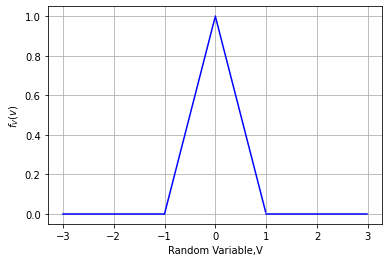
\includegraphics[scale=0.6] {Assignment_3_Fig_1.png}
    \caption{The PDF of V}
    \label{fig:The PDF of V}
\end{figure}
\end{frame}

\begin{frame}
 \frametitle{Solution Contd.}
 The CDF of V is defined as,
\begin{equation}
    F_V(v) = \pr{V \leq v}
\end{equation}
Now for $ v \le 0 $,
 \begin{align}
    \pr{V\leq v} &=  \int_{-\infty}^{v}f_{V}(v) \,dv  \\
          &=  \int_{-1}^{v} (1+v) \,dv  \\
          &=  \left(\dfrac{v^2}{2}+v \right) \Biggr|_{-1}^{v}  \\
          &=   \left(\left(\dfrac{v^2}{2}+v \right) - \left(\dfrac{1}{2} -1 \right)\right) \\
          &= \dfrac{v^2+2v +1}{2}
\end{align}
\end{frame}

\begin{frame}
 \frametitle{Solution Contd.}
 Similarly for $v \leq 1$,
\begin{align}
    \pr{V\leq v} &=  \int_{-\infty}^{v}f_{V}(v) \,dv  \\
          &=  \dfrac{1}{2} + \int_{0}^{v}(1-v)\,dv  \\
          &=  \dfrac{-v^2+2v+1}{2}
\end{align}
The CDF is as below: 
\begin{align}
\label{eq:cdf_v}
F_{V}(v)  = 
\begin{cases}
0 & v < -1
\\
\dfrac{v^2+2v + 1}{2} &  v \le 0
\\
\dfrac{-v^2+2v+1}{2} &  v \le 1
\\
1 & v > 1
\end{cases}
\end{align}
\end{frame}

\begin{frame}
\frametitle{Solution Contd.}
The plot for CDF of $V $ can be observed below.
\begin{figure}[!ht]
       \centering
    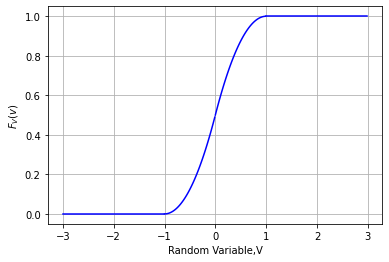
\includegraphics[scale=0.6] {Assignment_3_Fig_2.png}
    \caption{The CDF of V}
    \label{fig:The CDF of V}
\end{figure}
\end{frame}

\begin{frame}
\frametitle{Solution Contd.}
We need  $\pr{Z-W >\frac{1}{2}}$ where $Z = max(X,Y)$ and $W = min(X,Y)$. Now,
\begin{align}
Z-W  = 
\begin{cases}
X-Y & \text{for } X \geq Y
\\
Y-X & \text{for } X < Y
\end{cases}
\end{align}
\end{frame}

\begin{frame}
\frametitle{Solution Contd.}
 Therefore,
\begin{align}
    \pr{Z-W >\frac{1}{2}} &= \pr{X-Y>\frac{1}{2},X \geq Y}+\pr{Y-X >\frac{1}{2}, X < Y}\\
    &= \pr{X-Y>\frac{1}{2}} +\pr{Y-X>\frac{1}{2}}\\
    &= \pr{V > \frac{1}{2}} + \pr{-V > \frac{1}{2}}\\
    &= 1 - \pr{V \leq \frac{1}{2}} + \pr{V < \frac{-1}{2}}\\
    &= 1-F_V(\frac{1}{2}) + F_V(-\frac{1}{2})\\
    &= 1 -\frac{7}{8} + \frac{1}{8} \\
    &= \frac{1}{4} \implies \text{Option (3) is correct.} \nonumber
\end{align}   
\end{frame}

\end{document}
